\documentclass{thesis}
\usepackage{graphicx}
%\usepackage[dvipdfmx]{graphicx}
\usepackage[dvipdfmx]{color}
\usepackage{float}
\usepackage{listings}
\usepackage{jvlisting} %日本語のコメントアウトをする場合jvlisting(もしくはjlisting)が必要
\usepackage{amsmath}
\usepackage{mathtools}
\usepackage{stmaryrd} % \llparenthesis & rrparenthesis
\usepackage[dvipsnames]{xcolor}
\usepackage[hyphens]{url}
%\usepackage{hyperref}
\allowdisplaybreaks
%ここからソースコードの表示に関する設定
\lstset{
  basicstyle={\ttfamily},
  identifierstyle={\small},
  commentstyle={\smallitshape},
  keywordstyle={\small\bfseries\color{Green}},
  ndkeywordstyle={\small\color{orange}},
  stringstyle={\small\ttfamily\color{orange}},
  frame={tb},
  breaklines=true,
  columns=[l]{fullflexible},
  numbers=left,
  xrightmargin=10pt,
  xleftmargin=10pt,
  captionpos=b,
  numberstyle={\scriptsize},
  stepnumber=1,
  numbersep=0.5zw,
  lineskip=-0.3ex,
  keywords={At,Choreograhy2,Choreograhy3}, 
  %ndkeywords={com,select},% 追加のキーワードを指定
  moredelim=**[is][\color{gray}]{!}{!}, % 特定の要素を赤に設定
  moredelim=**[is][\color{red}]{|}{|},
  moredelim=**[is][\color{blue}]{`}{`}
}
%\usepackage{xcolor}
%%%%%%%%%%%%%%%%%%%%%%%%%%%%%%%%%%%%%%%%%%%%%%%%%%
%%% 基本設定

%目次を表示するには2回コンパイルが必要!!

\論文名{2024年度 卒業/修士論文}
\所属{岐阜大学大学院 自然科学技術研究科 知能理工学専攻 草刈研究室}
\学生番号{1224525023}
\氏名{恩田晴登}
\指導教員{草刈圭一朗}
\題目{Pythonの静的型検査器を活用したコレオグラフィックプログラミング言語の実装}
\日付{2024年2月5日}

%%%%%%%%%%%%%%%%%%%%%%%%%%%%%%%%%%%%%%%%%%%%%%%%%%
%%% ユーザ定義

% …… ご自由に定義してください ……
\renewcommand{\lstlistingname}{Code}
\newcommand{\projection}[2]{{\color{cyan}\llparenthesis}#1{\color{cyan}\rrparenthesis^#2}}
\newcommand{\mblue}[1]{\textbf{\textsf{\color{MidnightBlue}#1}}}
\newcommand{\cyan}[1]{\color{cyan}#1}
\newcommand{\gr}[1]{\color{ForestGreen}#1}
\newcommand{\nl}[1]{{\color{red}{\llbracket}}#1{\color{red}{\rrbracket}}} % Normalizer symbol
\newcommand{\mg}{~{\color{red}{\sqcup}}~} % Merging symbol
%%%%%%%%%%%%%%%%%%%%%%%%%%%%%%%%%%%%%%%%%%%%%%%%%%
\setcounter{tocdepth}{2}
%%% 本文
\begin{document}
\bibliographystyle{jplain}
\maketitle %表紙
\frontmatter\tableofcontents\mainmatter %目次

%%%%%%%%%%%%%%%%%%%%%%%%%%%%%%%%%%%%%%%%%%%%%%%%%%%%%%%%%%%%%%%%%%%%%%%%%%%%%%%%%%%%%%%%%%%%%%%%%%%%%%%%%%%%%%%%%%%%%%%%
%%% はじめに
\chapter{はじめに}
%論証したいStatementを記述

一般的に,並行・分散プログラムは,デッドロック等の並行性に起因するエラーや非決定性問題の
発見と修正が困難であるため構築が難しい.この問題の解決手法の一つとして,\textsf{コレオグラフィ}が提唱されている.
コレオグラフィは並行に動作する複数参加者の連携手順をまとめたプログラムであり,コレオグラフィックプログラミング言語によって記述される.
well-formedなコレオグラフィからは、\textsf{エンドポイント射影}と呼ばれる操作により、各参加者のプログラムを生成できる.
生成された各参加者のプログラムはデッドロック等の並行性に起因するエラーがないことが理論的に保証されている.
先行研究であるChoralは,Javaを拡張したコレオグラフィックプログラミング言語の一つである.
しかし,機械学習やIoTの分野で盛んに使用されているPythonを拡張したコレオグラフィックプログラミング言語は
著者が知る限りはまだ提案されていない.

本研究では,Pythonをベースとしたコレオグラフィックプログラミング言語\textsf{PyChoral}を構築し,有用性を確かめる.
これにより,機械学習やIoTを扱うプロジェクトにおいて、Pythonで並行・分散プログラムが実装可能となることを目指す足がかりとする.
本研究の特徴はPythonの型検査器である\textsf{Mypy}の型検査結果を活用することである.
PyChoralの構文はPythonと同一であることから,PythonのIDEやライブラリを使うことができる.
よって,Pythonの標準的な仕組みを保ったまま,単一のプログラムで並行・分散プログラムを記述できるという点で可用性をもつ.

本論文の構成を以下に示す.まず,2章で本研究の前提知識となるコレオグラフィックプログラミングとMypyの概要を述べる.
3章では本研究で構築したコレオグラフィック言語であるPyChoralについて述べ,プログラミング例を示す.
4章ではPyChoralの設計と実装について述べる.
5章ではPyChoralを用いたアプリケーションを示し,Pychoralの有用性を確かめる.
6章で結論と今後の課題を述べる.
付録AにはPyChoralにおけるエンドポイント射影,マージ,正規化の全体像を示す.

PyChoralの実装,プログラミング例,アプリケーションのソースコードは以下から入手可能である.

$~~~~~~~~~~~~~~~~~~~~~~~~~~~~~~~~~$\url{https://github.com/onharu/mypytest}
%%%%%%%%%%%%%%%%%%%%%%%%%%%%%%%%%%%%%%%%%%%%%%%%%%%%%%%%%%%%%%%%%%%%%%%%%%%%%%%%%%%%%%%%%%%%%%%%%%%%%%%%%%%%%%%%%%%%%%%%%%%%%%%%%%%%%%%%%%%%%%%%%%%%%%%%%%%%%%%%%%%%%%%%%%
\chapter{前提知識・先行研究}
%%%%%%%%%%%%%%%%%%%%%%%%%%%%%%%%%%%%%%%%%%%%%%%%%%%%%%%%%%%%%%%%%%%%%%%%%%%%%%%%%%%%%%%%%%%%
\section{コレオグラフィとエンドポイント射影}
コレオグラフィ \cite{Choreographic}とは,並行に動作する複数の参加者の連携手順をまとめたプログラムである.
コレオグラフィに従った各エンドポイントのプログラムは,デッドロック等の並行性起因のエラーが起こる恐れを排除できる.
各エンドポイント(通信の参加者)のプログラムはエンドポイント射影 \cite{endpoint}により,自動的に抽出される.
%図\ref{cho}はコレオグラフィ及びそれに従った各エンドポイントの例である.まず,客が店員に対してお金\textsf{money}を払う.
%商品の価格\textsf{price}に対して払った額が多い場合は,店員から客へ\textsf{'thanks'}を返し,商品の価格\textsf{price}に対して払った額が少ない場合は,店員から客へ\textsf{'not enough'}を返を返す.
%\begin{figure}[H]
%  \centering
%  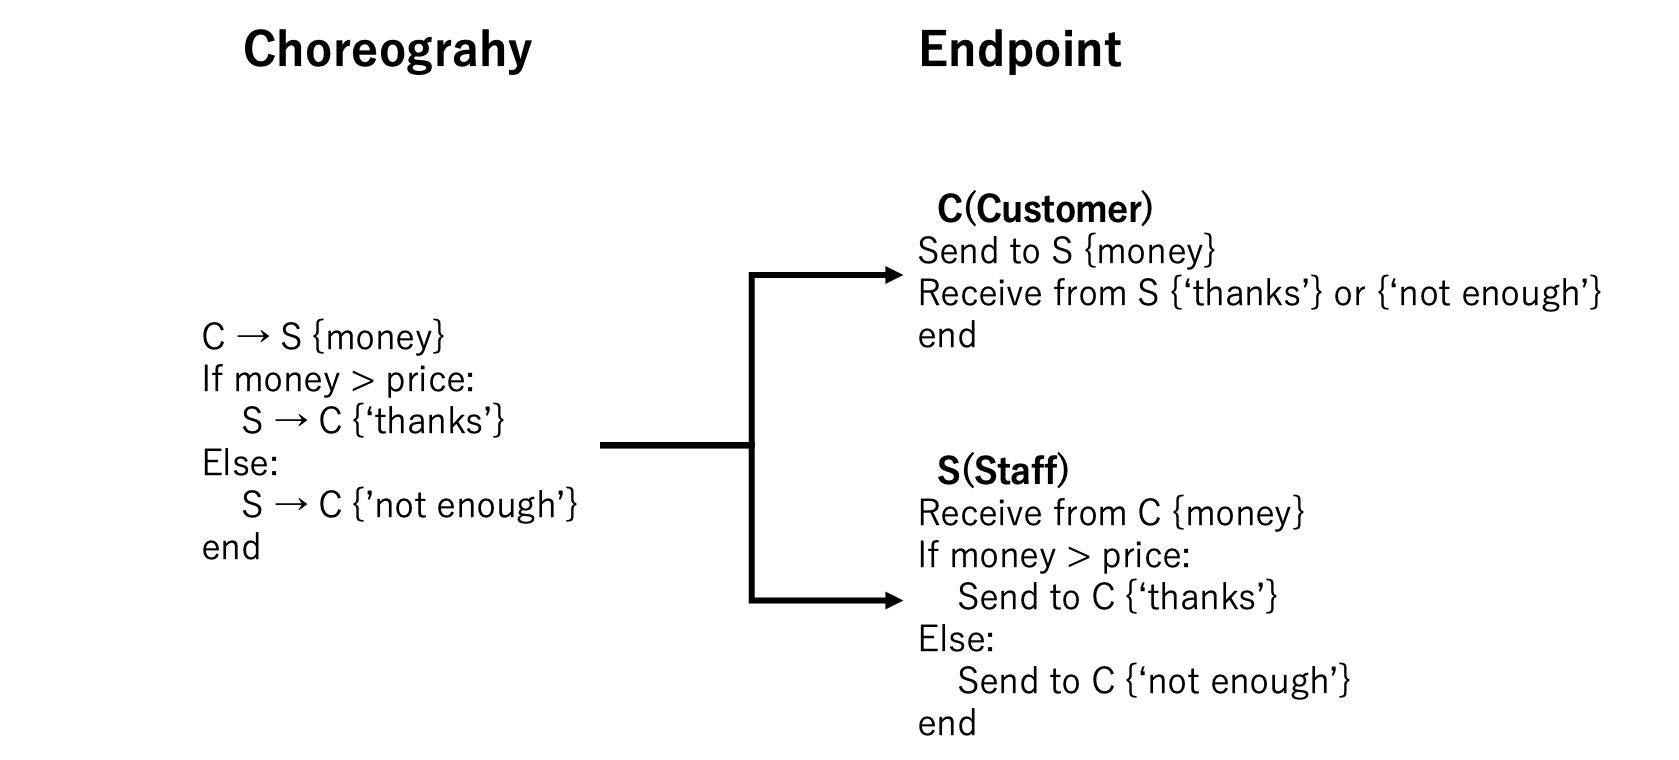
\includegraphics[scale=0.5]{image/cho.png}
%  \caption{コレオグラフィとエンドポイント(CustomerとStaffとの会計時の会話)}
%  \label{cho}
%\end{figure}

エンドポイント射影とは,コレオグラフィから各参加者のプログラムを導出する操作である.
コレオグラフィックプログラミング言語にはコンパイラが付属しており,コンパイラはエンドポイント射影理論によって並行に動作する実行可能なプログラムを出力する.

\begin{figure}[H]
  \centering
  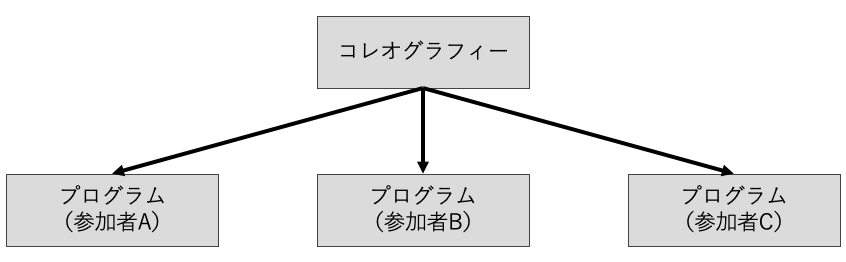
\includegraphics[scale=0.5]{image/epp.png}
  \caption{エンドポイント射影}
\end{figure}
%%%%%%%%%%%%%%%%%%%%%%%%%%%%%%%%%%%%%%%%%%%%%%%%%%%%%%%%%%%%%%%%%%%%%%%%%%%%%%%%%%%%%%%%%
\section{Choral}
Choral \cite{choral}はJavaをベースとしたコレオグラフィックプログラミング言語である.
Choralは,並行・分散システムに従わせたいプロトコル全体を単一のプログラムとして作成できるため,デッドロックが発生しないようにコーディングする必要があったプログラマの負担が軽減される.
Choralのオブジェクトには${\color{blue}{T@(R_1,\cdots,R_n)}}$という形式の型があり,Javaの基本的なオブジェクトインターフェイス$T$に
各参加者の情報となるパラメータ${\color{blue}{R_1,\cdots,R_n}}$が付随する.
これにより,Choralのコンパイラは独自のパーサーを使ってエンドポイント射影をする.この際に参加者の情報を含む型をもとに,各参加者のプログラムをコレオグラフィに従った形で自動的に生成することができる.
%これにより,Choralプログラムをコンパイルする際に各参加者のプログラムが,コレオグラフィに従った形で自動的に生成することができる.
%Code \ref{choral}はClient,Service,IPの3つの役割からなる分散認証システムを簡約したものである.
%Choralプログラムはクラス名や変数,型などに$@$で参加者名の情報を加えている.
%また,Choralにはcomメソッドとselectionメソッドなるものがある\cite{objective_Choreographies}.
%
%\begin{lstlisting}[caption=データ転送のための基本的な有向チャンネル,label=com]
%interface DiDataChannel@(A,B)<T@C> {
%  <S@D extends T@D> S@B com(S@A m);
%} 
%\end{lstlisting}
%Code \ref{com}はcomメソッドの最も簡易的に使用しているインターフェースの例である.DiDataChannelは,
%AとBで抽象化された2つの参加者間の有向チャンネルで,型パラメータTで抽象化された型のデータをAからBに転送するための
%インターフェースである.データ転送はcomを呼び出すことによって実行される.comは,Aに位置するTのサブタイプの任意の値S@Aを取り,S@Bを返す.
%例えばCode \ref{choral}の8行目の外側のcomはClientからIPへString型のメッセージ(credentional@IP.getsalt(...))を転送することを意味する.
%\begin{lstlisting}[caption=selectionメソッドの定義,label=select]
%interface DiSelectChannel@(A,B) {
%  @SelectionMethod
%  <T@C extends Enum@C<T>> T@B select(T@A m);
%} 
%\end{lstlisting}
%selectionメソッドは参加者間で列挙型のインスタンスを送信する際に使用する.
%%例えば,Code \ref{choral}の11行目,18行目ではClientからIPへ列挙型の値OK,KOを転送することを意味する.
%selectionメソッドは選択を意味し,プロジェクション後はswitch文に変換されてJavaプログラムが生成される.
%Choralは独自のパーサーにより,Choralプログラムからコンパイラを通して各エンドポイントのJavaプログラムが自動導出される.
それぞれのJavaプログラムはコレオグラフィに従っているため,相互関係によるバグがないことが保証されている.
これは,マルチパーティなプログラムを記述するJavaプログラマにとっては大きなメリットである.

%%%%%%%%%%%%%%%%%%%%%%%%%%%%%%%%%%%%%%%%%%%%%%%%%%%%%%%%%%%%%%%%%%%%%%%%%%%%%%%%%%%%%%%%%%%%%%%%%%%%%%%%%%%%%%
\newpage
\section{Mypy}
%\begin{itemize}
%  \item MypyはPythonの静的型検査器であり,既存のPythonコードに型アノテーションを追加することで,型が誤っていると警告を出すようになる.
%  \item Pythonは動的型付け言語であるため実行時にのみエラーが表示されるが,Mypyにより実行しなくてもコンパイル時にバグが検出できる.
%  \item Mypyの仕組み(プログラム→AST→型検査→エラー)← 図でやる
%\end{itemize}
%Pythonは動的型付け言語で実行時にのみエラーが表示されるので,コンパイル時に型に対するエラーは表示されない.
Mypy \cite{Mypy}はPythonの静的型検査器であり,既存のPythonコードに型注釈を追加することで,プログラムの実行前に型エラーを検出する.
これにより,コンパイル時にバグの検出が可能になり,安全なコーディングが可能となる.
\begin{lstlisting}[caption=型注釈のないPythonコード,numbers=none]
 def greeting(name):
   return 'Hello ' + name
 
 greeting(123)
 greeting(b'Alice')
\end{lstlisting}
\begin{lstlisting}[caption=型注釈のあるPythonコード,label=exmypy,numbers=none]
 def greeting(name: str) -> str:
   return 'Hello ' + name
 
 greeting('World')  # No error
 greeting(3)         
 |# Argument 1 to 'greeting' has incompatible type 'int'; expected 'str'|
 greeting(b'Alice')  
 |# Argument 1 to 'greeting' has incompatible type 'bytes'; expected 'str'|
\end{lstlisting}
%本研究ではMypyを別のPythonアプリケーションに統合するために,PythonプログラムにMypy.apiをインポートして型検査を行う.
図\ref{mypyproc}はMypyを使用した際の型検査のプロセスである.
Mypyはプログラムを一度抽象構文木に変換し,構文木を探索しながら型エラーがないか検査を行う.
型検査の結果はコンパイル終了時にテキストエディタに表示される(Code \ref{exmypy}).
\begin{figure}[H]
  \centering
  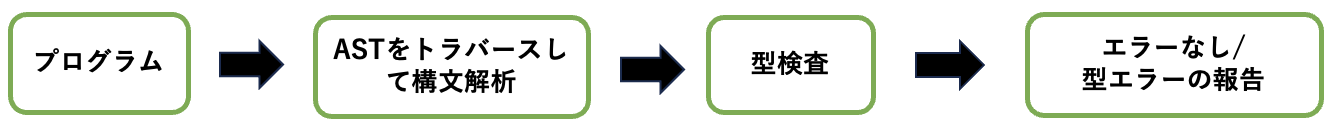
\includegraphics[scale=0.6]{image/mypyprocess.png}
  \caption{Mypyプロセス}
  \label{mypyproc}
\end{figure}

%%%%%%%%%%%%%%%%%%%%%%%%%%%%%%%%%%%%%%%%%%%%%%%%%%%%%%%%%%%%%%%%%%%%%%%%%%%%%%%%%%%%%%%%%%%%%%%%%%%%%%%%%%%%%%%%%%%%%%%%%%%%%%%%%%%%%%%%%%%%%%%%%%%%%%%%%%%%%%%%%%%%%%%%%%
\chapter{PyChoralによるプログラミング}
PyChoralはPythonベースのコレオグラフィックプログラミング言語である.
PyChoralはPythonの構文や型システムを踏襲して構築されている.
PyChoralを使用するコレオグラフィはプログラムのトップレベルにクラス定義を置き,それを用いて構築する.
通信の参加者間では,コレオグラフィの中でコレオグラフィの中で生成するチャネルを用いて通信をする.

Code \ref{pychoral}は,参加者Aから参加者Bに入力した整数値が2で割り切れる回数を伝達するコレオグラフィである.
AとBはそれぞれ\textsf{div2}メソッドを呼ぶ.Aには整数値\texttt{num}と割った回数をカウントする値\texttt{count}を引数として送る.
整数値\texttt{num}が2で割り切れる限り,\texttt{num}を2で割って,割った回数をカウントする.
割り切れなくなった場合は,それまでにカウントした回数をAからBへ伝える.
このコレオグラフィをユーザー側で使用するときは以下のようなプログラムになる.
回数を数える変数\texttt{count}は0に指定する.nは任意の整数値を代入できる.例えば,$n=8$の場合はBに整数値3が伝わる.$n=-3$の場合はに整数値0が伝わる.

\begin{lstlisting}[numbers=none]
 # A
 div_a = Divide2_A()
 div_a.divide_by_two(n,0)
 # B
 div_b = Divide2_B()
 div_b.divide_by_two()
\end{lstlisting}
1行目はクラス定義であり,型パラメータ\texttt{A}および\texttt{B}が通信の参加者となる.
2,3行目はクラスのコンストラクタを表す.ここではAからBへobject型の値を送るチャネル\texttt{chAB}を生成している.
このプログラムではAからBへ列挙型の\texttt{OddEven}とint型のカウント数\texttt{count}を送る場合があるため,どちらの型
も送信できるようにobject型でコンストラクタを生成する.

4-10行目はAとBが連携して動作するメソッド\texttt{divide\_by\_two}である.
メソッドの引数\texttt{num,count}は参加者Aがもつint型の値であり,戻り値は参加者Bがもつint型の値である.
5行目のif文では,Aがもつ整数\texttt{num}が2で割り切れるかどうかで分岐する.この分岐の結果はまだBには知らされない.
6,7行目は割り切れる場合,9,10行目は割り切れない場合である.
6,9行目では\texttt{select}メソッドにより条件分岐の結果を示す列挙型の値をAからBへ送っている.
%6,9行目にある\texttt{select}は条件分岐の結果を示す列挙型の値を送るメソッドである.
6行目では\texttt{num}が偶数であるということを知らせる列挙型の値{\color{red}{\texttt{EVEN}}}をBへ送っている.
9行目では\texttt{num}が奇数であるということを知らせる列挙型の値{\color{blue}{\texttt{ODD}}}をBへ送っている.
7行目では,メソッド\texttt{divide\_by\_two}の引数に,\texttt{num}を2で割った値と1だけ加算されたカウント数を引数として再帰呼び出しをしている.
10行目では\texttt{com}メソッドによりカウントした整数値をAからBへ送っている.
%\texttt{com}は送信者の情報を含む任意の型をもつ値を送るメソッドである.

\begin{lstlisting}[caption = 参加者\texttt{A,B}のコレオグラフィ,label=pychoral]
 class Divide2(Choreograhy2[A,B]):
    def __init__(self) -> None:
       self.chAB : Channel[object,A,B] = Channel[object,A,B]('A','B')
    def divide_by_two(self,num:At[int,A],count:At[int,A]) -> At[int,B]:
       if (num % 2@A())@A() == 0@A():
           self.chAB.select(|OddEven.EVEN|@A())
           return self.divide_by_two((num // 2)@A(),(count + 1)@A())
       else:
           self.chAB.select(`OddEven.ODD`@A())
           return self.chAB.com(count@A())
\end{lstlisting}

クラス\texttt{Divide2(Choreograhy2[A,B])}からエンドポイント射影により,クラス\texttt{Divide2\_A},\texttt{Divide2\_B}が生成される.
参加者A,Bはプロセスから\texttt{Divide2\_A},\texttt{Divide2\_B}のメソッド\texttt{divide\_by\_two}を呼び出すことにより連携して動作する.
%Code \ref{pythonA}は,Code \ref{pychoral}から射影されたAのPythonプログラムである.
%Code \ref{pythonB}は,Code \ref{pychoral}から射影されたBのPythonプログラムである.
Code \ref{pythonA}とCode \ref{pythonB}は,Code \ref{pychoral}からエンドポイント射影された各参加者のPythonプログラムである.
型注釈,それぞれの参加者が関連しない式や文は除去される.
\begin{lstlisting}[caption = 参加者APythonプログラム, label = pythonA]
 class Diveide2_A():
     def __init__(self):
         self.chAB = Channel[object,A,B]('A','B')
     def divide_by_two(self,num,count):
         if (num % 2) == 0:
             Unit.id(self.chAB.select(|OddEven.EVEN|))
             return Unit.id(self.divide_by_two(num // 2, count + 1))
         else:
             Unit.id(self.chAB.select(`OddEven.ODD`))
             return Unit.id(self.chAB.com(count))
 \end{lstlisting}
 
 \begin{lstlisting}[caption = 参加者BのPythonプログラム, label = pythonB]
 class Divide2_B():
     def __init__(self):
         self.chAB = Channel[object,A,B]('A','B')
     def divide_by_two(self):
         match self.chAB.select():
             case |OddEven.EVEN|:
                 return self.divide_by_two()
             case `OddEven.ODD`:
                 return self.chAB.com()
             case _:
                 raise Exception
\end{lstlisting}

参加者Aはチャネル\texttt{chAB}を介してBに値を送るため,\texttt{select}や\texttt{com}などのメソッド呼び出しでは戻り値がない.
そのため,Code \ref{pythonA}の6行目以降に出てくるメソッド呼び出しは全て\texttt{Unit}値となっている.

条件分岐を含むコレオグラフィのエンドポイント射影で重要なのは,ある参加者で発生した条件分岐を
いかにして他の参加者に伝えるか,という仕組みを実現することである.これを実現するのが\textbf{マージ}である.
PyChoralにおけるエンドポイント射影およびマージの理論はChoralを模倣している.
if文におけるマージは,if文の条件式を判断した参加者以外が条件式の結果に相当する列挙型の値を受信して分岐することにより実現する.
PyChoralではPython3.10から導入されたmatch文を使用している.
match文のケースはCode \ref{pychoral}の6,9行目にある\texttt{select}メソッドで送信した列挙型の値で分ける.
Code \ref{pychoral}の6行目から射影によりCode \ref{pythonB}の5-7,10行目が生成される.
Code \ref{pychoral}の9行目からは射影によりCode \ref{pythonB}の5,8-10行目が生成される.
\texttt{case \_} は共通のケースであるため,統合されて一つになる.
\texttt{{\color{red}{OddEven.EVEN}},{\color{blue}{OddEven.ODD}}}は独立したケースであるため,マージ後のmatch文にそのまま加える.
\begin{figure}[H]
  \centering
  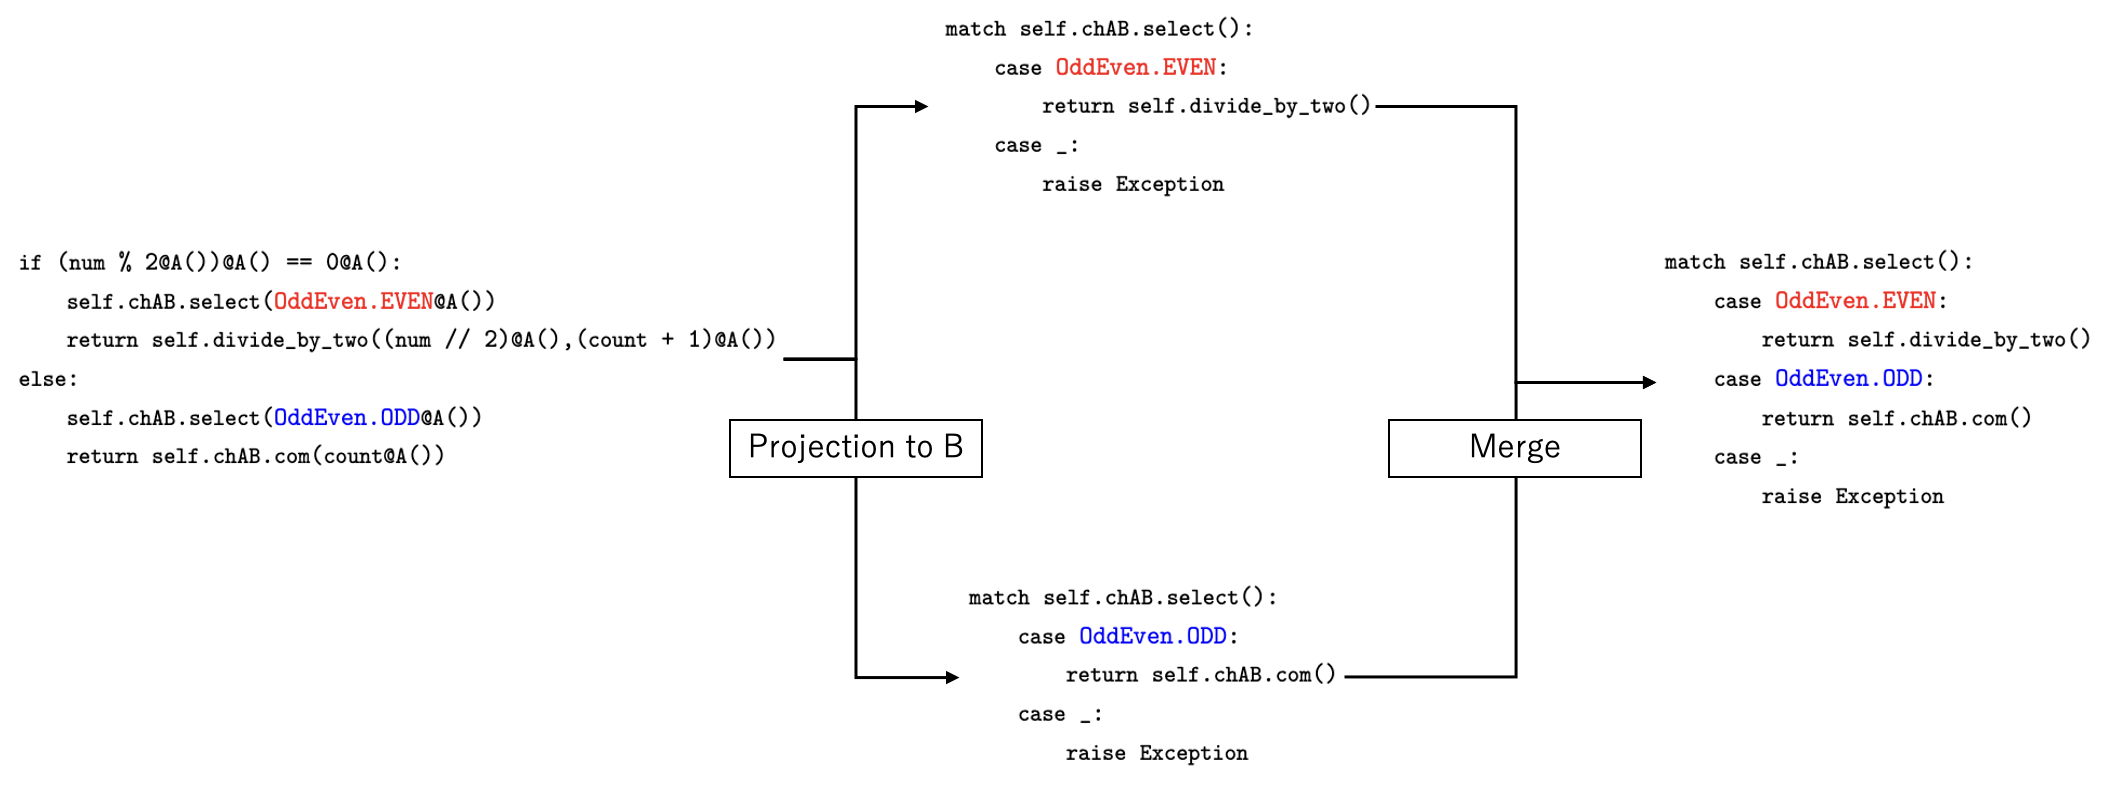
\includegraphics[scale=0.413]{image/merge.png}
\end{figure}

これにより,条件分岐に関係ない参加者も分岐を考慮した形でエンドポイント射影される.
生成されたA,BのPythonプログラムは,エンドポイント射影およびマージによりデッドロックが起こることなく連携して動作することが可能である.
%%%%%%%%%%%%%%%%%%%%%%%%%%%%%%%%%%%%%%%%%%%%%%%%%%%%%%%%%%%%%%%%%%%%%%%%%%%%%%%%%%%%%%%%%%%%%%%%%%%%%%%%%%%%%%%%%%%%%%%%%%%%%%%%%%%%%%%%%%%%%%%%%%%%%%%%%%%%%%%%%%%%%%%%%%
\chapter{PyChoralの設計と実装}
この章ではPyChoralの構文およびエンドポイント射影の設計について述べる.その後,その設計をもとに本研究の実装について述べる.
%%%%%%%%%%%%%%%%%%%%%%%%%%%%%%%%%%%%%%%%%%%%%%%%%%%%%%%%%%%%%%%%%%%%%%%%%%%%%%%%%%%%%%%%%%%%%%%%%%%%%%%%%%%%%%%%%%%%%%%%%%%%%%%%%%%%%%%%%%%%%%%%%%%%%%%%%%%%%%%%%%%%%%%%%%
\section{PyChoralの構文とエンドポイント射影の定義}
PyChoralの構文はPythonと同一である.図 \ref{syntax}はPythonの構文定義である.
プログラムの構文木はトップレベルからクラス定義(\textsf{Class}),関数およびメソッド定義(\textsf{FuncDef}),文(\textsf{Stm}),式(\textsf{Exp})のいずれかの構文要素で構成される.
PyChoralでは全ての式に参加者の情報が割り当てられる.
参加者の情報はPythonの基本型とともに{\color{Green}{Typed Annotation}}で表現されるか,リテラル値に\mblue{@}をつけて表現される.
オーバーラインが引かれている$Exp$や$Stm$などはそれらのリストを表す.
\begin{figure}[H]
  \centering
  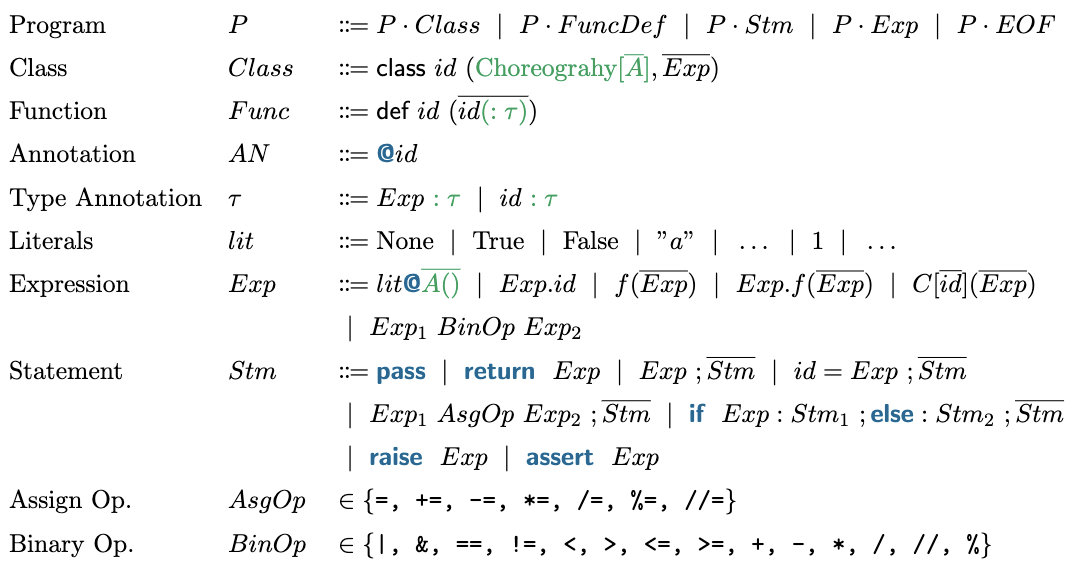
\includegraphics[scale=0.8]{image/syntax.png}
  \caption{Syntax of PyChoral}
  \label{syntax}
\end{figure}
%%%%%%%%%%%%%%%%%%%%%%%%%%%%%%%%%%%%%%%%%%%%%%%%%%%%%%%%%%%%%%%%%%%%%%%%%%%%%%%%%%%%%%%%%%%%%%%%%%%%%%%%%%%%%%%%%%%%%%%%%%%%%%%%%%%%%%%%%%%%%%%%%%%%%%%%%%%%%%%%%%%%%%%%%%
PyChoralはエンドポイント射影において型情報を活用する.
これは,すべての式や文が射影される参加者と関連するかどうかに基づいて射影をするためである.
エンドポイント射影の設計は構文木の項\textsf{Term}と射影先の参加者\textsf{R}をとり,同じ構文をもつ項へ移す写像とする.
とあるコレオグラフィの参加者$\cyan{\text{A}}$に対するPyChoralの項のエンドポイント射影は$\projection{\textsf{Term}}{A}$と記し,参加者$\cyan{\text{A}}$の振舞いを表すPythonの項となる.
PyChoralの構文に無く,安全でないプログラムを射影する場合は未定義としてエラーが出力される.
%
%クラス定義の射影はクラス継承の第一引数Chクラスに存在する参加者名によってPythonの項を生成する.
%\begin{alignat*}{2} 
%  &\projection{\textsf{class} ~id~(Ch[\overline{\cyan{R}}],\overline{Exp}):\overline{Stm}}{A}=
%  \begin{cases}
%    \textsf{class} ~id\_{\cyan{A}}~(\overline{\projection{Exp}{A}}):\overline{\projection{Stm}{A}} & \text{if}~~ {\cyan{A}} \in \overline{\cyan{R}}\\
%    \text{absent} & \text{if}~~ {\cyan{A}} \notin \overline{\cyan{R}}
%  \end{cases}
%\end{alignat*}
%(例)参加者$\cyan{\text{A}},\cyan{\text{B}}$が関わるクラス$\textsf{Foo}$の射影
%\begin{alignat*}{2} 
%  &~~~~~~~~~\textsf{PyChoral} ~~~~~~~~~~~~~\Longrightarrow~~~~~~ \textsf{Python}\\
%  &\projection{\textsf{class} ~\text{Foo} \text{(Ch2[{\cyan{A}},{\cyan{B}}])}}{A} ~~~\Longrightarrow~~~ \textsf{class} ~\text{Foo\_{\cyan{A}}}(~)\\
%  &\projection{\textsf{class} ~\text{Foo} \text{(Ch2[{\cyan{A}},{\cyan{B}}])}}{B} ~~~\Longrightarrow~~~ \textsf{class} ~\text{Foo\_{\cyan{B}}}(~)\\
%  &\projection{\textsf{class} ~\text{Foo} \text{(Ch2[{\cyan{A}},{\cyan{B}}])}}{C} ~~~\Longrightarrow~~~ 
%\end{alignat*}
%
%関数定義は引数の型注釈に射影される参加者の情報があればその引数を残す.
%\begin{alignat*}{2} 
%  &\projection{\textsf{def} ~id~(\overline{id:TE}):\overline{Stm}}{A} = \textsf{def} ~id~ (\overline{id}):\overline{\projection{Stm}{A}}\\
%\end{alignat*}
%(例)参加者$\cyan{\text{A}}$が関連する引数をもつ関数\text{f}の射影
%%参加者$\cyan{\text{A}}$に対して関数定義$\textsf{def}~f(x:\text{At[int,{\cyan{A}}]})$から射影された関数は$\textsf{def}~f(x)$となり,$\textsf{def}~f(x:\text{At[int,{\cyan{B}}]})$から射影された関数は$\textsf{def}~f()$となる.
%\begin{alignat*}{2} 
%  &~~~~~~~~~~~\textsf{PyChoral} ~~~~~~~~~~~~~~~\Longrightarrow~~~~~~ \textsf{Python}\\
%  &\projection{\textsf{def} ~\text{f}~(\text{self},x:\text{At[int,{\cyan{A}}]})}{A} ~~~\Longrightarrow~~~ \textsf{def} ~\text{f}~ (\text{self},x)\\
%  &\projection{\textsf{def} ~\text{f}~(\text{self},x:\text{At[int,{\cyan{A}}]})}{B} ~~~\Longrightarrow~~~ \textsf{def} ~\text{f}~ (\text{self})\\
%\end{alignat*}
%
%式 Expression は射影する際に文字列を生成する($\text{Expression} \rightarrow \text{String}$).
%リテラルは$@$を付けることで関係する参加者を判別可能である.射影される参加者の情報がある場合はリテラルをそのまま生成し,ない場合はUnit値が生成される.
%\begin{alignat*}{2} 
%  &\projection{lit\mblue{@}(\overline{{\color{cyan}{B}}()}):\tau}{A}=
%  \begin{cases}
%    lit & \text{if}~~ {\color{cyan}A} \in \overline{\color{cyan}{B}}\\
%    \texttt{Unit.id} &\text{otherwise}
%  \end{cases}\\
%\end{alignat*}
%(例)$123@{\cyan{\text{A}}}()$の射影
%\begin{alignat*}{2} 
%  &\projection{123\mblue{@}{\color{cyan}{A}}()}{A} = 123\\
%  &\projection{123\mblue{@}{\color{cyan}{A}}()}{B} = \texttt{Unit.id}
%\end{alignat*}
%その他の式は型注釈や型推論から参加者の情報を取得し,各定義によって射影される.
例えば,メソッド呼び出し( $Exp_1.f(\overline{Exp_2})$ )はレシーバオブジェクト$Exp_1$,引数$\overline{Exp_2}$および
メソッド呼び出しの戻り値の型情報に射影される参加者の情報があるかどうかで場合分けをする.以下はメソッド呼び出しのエンドポイント射影の定義である.
\begin{alignat*}{2} 
  &\projection{Exp_1.f(\overline{Exp_2}):\tau}{A}=
  \begin{cases}
    \projection{Exp_1}{A}.f(\overline{\projection{Exp_2}{A}}) \\
    ~~~~~~~~~~~~~~~~~~~\text{if}~~ {\color{cyan}A} \in \text{rolesOf}(Exp_1) \wedge {\color{cyan}A} \in \text{rolesOf}(\overline{Exp_2})\\
    ~~~~~~~~~~~~~~~~~~~~~~~~~~~~~~~~~~~~~~~~~~ \wedge {\color{cyan}A} \in \text{rolesOf}(Exp_1.f(\overline{Exp_2}))\\
    \texttt{Unit.id}(\projection{Exp_1}{A}.f(\overline{\projection{Exp_2}{A}})) \\
    ~~~~~~~~~~~~~~~~~~~\text{if}~~ {\color{cyan}A} \in \text{rolesOf}(Exp_1) \wedge {\color{cyan}A} \notin \text{rolesOf}(Exp_1.f(\overline{Exp_2}))\\
    \texttt{Unit.id}(\projection{Exp_1}{A},\overline{\projection{Exp_2}{A}}) ~~~~~\text{otherwise}
  \end{cases}\\
\end{alignat*}
メソッド呼び出しの場合分けに出てくる$\textsf{rolesOf(~)}$とは,式の型情報を参照し,その型から参加者の情報を文字列の集合として返す関数である.
戻り値の型情報に射影先の参加者が含まれていない場合は\textsf{Unit}値を返す.レシーバオブジェクトや引数はそれぞれ再帰的に射影される.
例えば,Code \ref{pychoral}の10行目にあるメソッド呼び出し$\texttt{self.chAB.com(count@A())}$は参加者A,Bに対して以下のように射影され,Pythonのプログラムとして生成される.
この例の場合,$\textsf{rolesOf}(Exp_1) = \{\text{A,B}\}$, $\textsf{rolesOf}(\overline{Exp_2}) = \{\text{A}\}$, $\textsf{rolesOf}(Exp_1.f(\overline{Exp_2})) = \{\text{B}\}$である.
\begin{alignat*}{2} 
  &\projection{\texttt{self.chAB.com(count@A())}}{A} &&~\Longrightarrow~ \texttt{Unit.id}(\projection{\texttt{self.chAB}}{A}\texttt{.com}(\projection{\texttt{count@A()}}{A})) \\
  &&&~\Longrightarrow~ \texttt{Unit.id}(\texttt{self.chAB.com(count)})\\
  \\
  &\projection{\texttt{self.chAB.com(count@A())}}{B} &&~\Longrightarrow~ \projection{\texttt{self.chAB}}{A}\texttt{.com}(\projection{\texttt{count@A()}}{A}) \\
  &&&~\Longrightarrow~ \texttt{self.chAB.com(Unit.id)}\\
  %&\projection{\texttt{self.chAB.com(count@A())}}{B} ~\Rightarrow~ \text{ChAB.com(\texttt{Unit.id})}\\
  %&\projection{\texttt{self.chAB.com(count@A())}}{C} ~\Rightarrow~ \texttt{Unit.id}(\texttt{Unit.id},\texttt{Unit.id})
\end{alignat*}
次に,3章で述べた条件分岐によるエンドポイント射影とマージの定義について述べる.
文\textsf{Stm}は,文中に現れる式や文をそれぞれ射影する形式を取る.例えばreturn文のエンドポイント射影は
$\projection{\mblue{return} ~ Exp}{A} = \mblue{return} ~ \projection{Exp}{A}$となり,
戻り値である式$Exp$のエンドポイント射影が再帰で行われたreturn文が新しくPythonプログラムとして生成される.
しかし,\textsf{select}メソッド呼び出しの式文とif文は,他の文とエンドポイント射影の形式が異なる.

%式文のエンドポイント射影を以下のように定義する.
メソッド呼び出し以外,またはメソッド名が\textsf{select}以外のメソッド呼び出しである式文は,他の文と同じように再帰的に射影されていく.
\textsf{select}メソッド呼び出しの式文である場合は,\textsf{match}文に射影される.\textsf{select}メソッドは引数に列挙型の値\texttt{id}をとり,その値は射影されたmatch文での場合分けに使用する.
この場合を満たさない場合は,ワイルドカードを用いて例外とする.
\begin{alignat*}{2} 
  &\projection{Exp~;\overline{Stm}}{A} =
  \begin{cases}
    \mblue{match} ~\projection{Exp}{A}: \\
    ~~~~~\mblue{case} ~id: \projection{\overline{Stm}}{A};~~~~~~~~~~~ \text{if}~~Exp = Exp_1.\texttt{select}(id\mblue{@}{\cyan{A}}()),~ id:\texttt{Enum}\\ %~~~ \text{Name}(f) = \texttt{Select}\\%&~~~~ {\cyan{A}} \in \text{rolesOf}(Exp.f(\overline{Exp})) ~~\text{and}\\
    ~~~~~\mblue{case} ~\_\_: \text{raise Exception}; \\
    \projection{Exp}{A};\projection{\overline{Stm}}{A} ~~~~~~~~~~~~~~~~~~ \text{otherwise}\\
  \end{cases}
\end{alignat*}

if文は,条件式$Exp$の型情報に射影先の参加者が含まれる場合,そのままif文の構文を保ったまま再帰的に射影が行われていく.
そうでない場合は,条件分岐の結果がどうなろうと振舞えるようにするために,then節とelse節に存在する後続の文を正規化(${\color{red}{\llbracket}}~{\color{red}{\rrbracket}}$)し,マージ($~{\color{red}{\sqcup}}~$)する必要がある.
\begin{alignat*}{2} 
  &\projection{\mblue{if}~Exp:Stm_1~;\mblue{else}:Stm_2 ~;\overline{Stm}}{A}=\\
  &
  ~~~~~~~~~~~\begin{cases}
    \mblue{if}~\projection{Exp}{A} : \projection{Stm_1}{A} ~; \mblue{else}:\projection{Stm_2}{A} ~;\projection{\overline{Stm}}{A} & \text{if}~~ \text{rolesOf}(Exp) = \cyan{A}\\
    \projection{Exp}{A} ~; \nl{\projection{Stm_1}{A}} \mg \nl{\projection{Stm_2}{A}} ~;\projection{\overline{Stm}}{A} & \text{otherwise}
  \end{cases}\\
\end{alignat*}
マージ演算子$\mg$は,分岐のプログラムを結合する演算子である.\textsf{match}文以外のマージは,結合されるPythonプログラムの式,文は等価であるとする.
2つのmatch文のマージは,$Exp$のマージを条件式とするmatch文となる.各caseに関して,両方に存在する各ケースは元のケース
に続く文($Stm_a,...$)をマージしたケースを得る.片方にしかないケースはマージ後のmatch文にそのまま加える.
\begin{alignat*}{2} 
  & \mblue{match}~Exp: ~~~~~~~~~~~~~~~~~~~~\mblue{match}~Exp': ~~~~~~~~~~~~~~~~~~~~\mblue{match}~Exp \mg Exp':\\
  & ~~~\mblue{case}~id_a : Stm'_a; ~~~~~~~~~~~~~~~~\mblue{case}~id_a : Stm''_a; ~~~~~~~~~~~~~~~~\mblue{case}~id_a : Stm'_a \mg Stm''_a;\\
  & ~~~\cdots ~~~~~~~~~~~~~~~~~~~~~~~~~~~~~~~~~\cdots ~~~~~~~~~~~~~~~~~~~~~~~~~~~~~~~~~~\cdots\\
  & ~~~\mblue{case}~id_x : Stm'_x; ~~~~~~\mg~~~~~~\mblue{case}~id_x : Stm''_x; ~~~~~~=~~~~~~\mblue{case}~id_x : Stm'_x \mg Stm''_x;\\
  & ~~~\mblue{case}~id_y : Stm'_y; ~~~~~~~~~~~~~~~~~~~~~~~~~~~~~~~~~~~~~~~~~~~~~~~~~~~~~~\mblue{case}~id_y : Stm'_y; \\
  & ~~~~~~~~~~~~~~~~~~~~~~~~~~~~~~~~~~~~~~~~~\mblue{case}~id_z : Stm'_z;~~~~~~~~~~~~~~~~\mblue{case}~id_z : Stm'_z;\\
  & ~~~\mblue{case}~~\_\_ ~: Stm'_{ex}; ~~~~~~~~~~~~~~~\mblue{case}~~\_\_ ~: Stm''_{ex}; ~~~~~~~~~~~~~~~\mblue{case}~~\_\_ ~:Stm'_{ex} \mg Stm''_{ex};\\
\end{alignat*}


%\begin{lstlisting}[caption=射影前のプログラム,label=1]
%if valid: #@IP
%  ch_Client_IP.select(AuthBranch.OK@IP())
%  ch_Service_IP.select(AuthBranch.OK@IP())
%  ...
%  return AuthResult[Client,Service](ch_Client_IP.com(t), ch_Service_IP.com(t))
%else:
%  ch_Client_IP.select(AuthBranch.KO@IP())
%  ch_Service_IP.select(AuthBranch.KO@IP())
%  return AuthResult[Client,Service]()
%\end{lstlisting}
%if文の射影の定義により,条件式が射影される参加者と関係ないためCode \ref{2}となり,これらがマージされてCode \ref{3}となる.
%$\projection{Exp}{A} ~; \nl{\projection{Stm_1}{A}} \mg \nl{\projection{Stm_2}{A}} ~;\projection{\overline{Stm}}{A}$の$\nl{\projection{Stm_1}{A}}$部分にあたるのがCode \ref{2}のOKの場合であり,$\nl{\projection{Stm_2}{A}}$部分にあたるのがCode \ref{2}のKOの場合である.
%\begin{lstlisting}[caption=射影後のプログラム(マージ前),label=2]
%#OK#
%match ch_Client_IP.select(Unit.id):
%  case OK:
%    return AuthResult(ch_Client_IP.com(Unit.id),Unit.id)
%  case __:
%    raise Exception
%
%# KO
%match ch_Client_IP.select(Unit.id):
%  case OK:
%    return AuthResult()
%  case __:
%    raise Exception
%  \end{lstlisting}
%\begin{lstlisting}[caption=射影後のプログラム(マージ後),label=3]
%match ch_Client_IP.select(Unit.id):
%  case OK:
%    return AuthResult(ch_Client_IP.com(Unit.id),Unit.id)
%  case OK:
%    return AuthResult()
%  case __:
%    raise Exception
%\end{lstlisting}
%また,マージされる後続のStatementはマージされる前に正規化される(詳細は付録A.3に記載).
%%%%%%%%%%%%%%%%%%%%%%%%%%%%%%%%%%%%%%%%%%%%%%%%%%%%%%%%%%%%%%%%%%%%%%%%%%%%%%%%%%%%%%%%%%%%%%%%%%%%%%%%%%%%%%%%%%%%%%%%%%%%%%%%%%%%%%%%%%%%%%%%%%%%%%%%%%%%%%%%%%%%%%%%%%%%%%%%%%%%%%%%%%%%%%%%%%%%%%%%%%%%%%%%%%%
\section{エンドポイント射影の実装}

4.1節で述べたエンドポイント射影を実現するために,PyChoralはPythonの基本型や型クラスに参加者の情報を含める形で拡張する.
具体的な手法は次の2つである.
\subsubsection*{型の拡張}
参加者の情報を含む型として\textbf{At[T1,R]}や\textbf{Choreograhy2[R1,R2]},\textbf{Choreograhy3[R1,R2,R3]}を定義する.
\texttt{At[T1,R]}は参加者Rに割り当てられる値の型\texttt{T1}を表す型である.
PyChoralにおける\texttt{At[T1,R]}はPythonの基本型\texttt{T1}と同様に扱える.
\texttt{Choreograhy2[R1,R2]},\texttt{Choreograhy3[R1,R2,R3]}はPyChoralプログラムでクラス宣言をする際に継承する基底クラスの型である.
型パラメータに参加者の情報をもち,参加者の人数で継承するクラスを指定する.
\texttt{At},\texttt{Choreograhy2},\texttt{Choreograhy3}の型パラメータはジェネリック型をとり,コレオグラフィでは任意の型をとれるプレースホルダとして機能する.
\begin{lstlisting}[frame = none, numbers = none]
class Choreograhy2(Generic[R1,R2]):
class Choreograhy3(Generic[R1,R2,R3]):
class At(Generic[T1,R],T1):
\end{lstlisting}

\subsubsection*{式の拡張}
Pythonのすべての式が属する型クラスである\textsf{object}型に\textbf{\mblue{@}演算子}を追加で定義する.
これにより,\texttt{Exp\mblue{@}R()}のように式\texttt{Exp}に参加者Rを割り当てることが可能となる.
ここで,\texttt{Exp}の型が\texttt{T1}であれば\texttt{Exp\mblue{@}R()}の型は\texttt{At[T1,R]}と解析される.
\begin{lstlisting}[frame =none,numbers = none]
class object:
    def __matmul__(self:Self, _:R1) -> At[Self,R1]: ...
\end{lstlisting}
\mblue{@}演算子および型クラス\texttt{At},\texttt{Choreograhy2},\texttt{Choreograhy3}はエンドポイント射影で参加者の情報を得るために用いられる.
これらを実体を持たないMypyの型宣言の形で定義することにより,各参加者のプログラムでは\mblue{@}演算子,型クラス\texttt{At,Choreograhy2,Choreograhy3}が消去される.%標準のPythonプログラムとして実行できる.

\texttt{Channel},\texttt{SymChannel}は2者間の通信をするメソッドをもつ型クラスである.
\texttt{Channel}は型パラメータ\texttt{R1}から\texttt{R2}へ\textsf{com}メソッドか\textsf{select}メソッドを使って通信するクラスである.
\texttt{SymChannel}は\texttt{@overload}デコレータを使用してオーバーロードを定義する.これにより,\texttt{R1}と\texttt{R2}との双方向通信を実現する.
\texttt{com}は送信者の情報を含む任意の型\texttt{At[T1,R1]}をもつ値\texttt{msg}を受信者に送るメソッドである.
\texttt{select}は送信者がもつ条件分岐の結果を示す列挙型の値を受信者へ送るメソッドである.
\begin{lstlisting}[numbers = none]
class Channel(Generic[T1,R1,R2]):
    def com(self,msg:At[T1,R1]) -> At[T1,R2]:
    def select(self,msg:At[T1,R1]) -> At[T1,R2]:

class SymChannel(Generic[T1,R1,R2]):
    @overload
    def com(self,msg:At[T1,R1]) -> At[T1,R2]:
    @overload
    def com(self,msg:At[T1,R2]) -> At[T1,R1]:
    @overload
    def select(self,msg:At[T1,R1]) -> At[T1,R2]:
    @overload
    def select(self,msg:At[T1,R2]) -> At[T1,R1]:
\end{lstlisting}


PyChoralではMypyを活用した型検査のプロセスを改造し,型検査を行なった後に各参加者の抽象構文木を再構築する.
射影後に再構築される構文木は新しいデータ構造を取り,それに従ったPythonプログラムが生成される.

\begin{figure}[H]
  \centering
  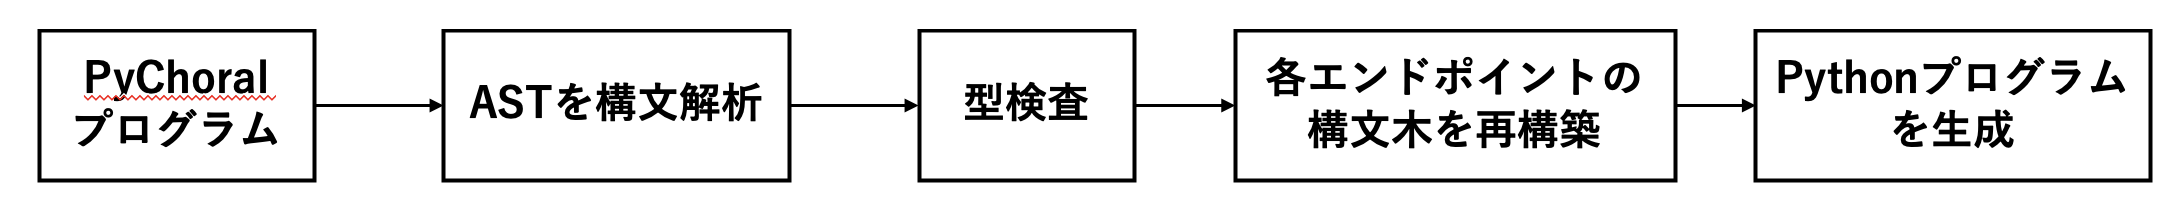
\includegraphics[scale=0.4]{image/pychoralprocess.png}
  \caption{PyChoralプロセス}
  \label{pychoralprocess}
\end{figure}
<Mypyの改造>

PyChoralはPythonベースの言語のため,JavaベースのChoralを模倣するには静的型付け言語として扱え,コンパイル時にエラーの有無を判別したい.そのため,Mypyを活用して静的に型をつける.
ただし,Mypyで型注釈をつけらればChoralと同じように動くかというと,そうではない.

まず,ChoralはJavaのパーサーを改良し,独自のコンパイラを使用してChoralプログラムからJavaプログラムを自動導出しているが,本研究では既存のPythonパーサーをそのまま活用する.
Choralはクラス定義,インターフェース,変数,型に$\mblue{@}$で参加者の情報を加えていたが,Mypyの型検査ではこれを認識しない.
この問題に対して,本研究では主に2つの方法で各参加者の情報をとることにした.

1つ目の方法として,Mypyが型検査する際に参照する標準ライブラリのtypeshedに\textsf{At,Channel}といった新たな型クラスを追加し,変数の型注釈に参加者情報を加えられるようにした.
\textsf{At,Channel}の引数はジェネリック型をとっており,任意の型を後から取ることができるプレースホルダーとして機能している.
例えばPyChoralのプログラム例(Code \ref{pychoral})の3行目にある$\texttt{price:At[int,S]}$は,変数$\text{price}$の型が$\text{int}$で参加者$\text{S(Staff)}$に関連する値ということが分かる.

2つ目の方法として,Mypyが型検査する際に参照されるobjectクラスに$\mblue{@}$のためのメソッド$\texttt{\_\_matmul\_\_}$を追加し,role.pyで各参加者に対して適用することで$\mathbf{123\mblue{@}A()}$
のように$\mblue{@}$をつけてプログラミングしてもMypyの型検査が通るようにした.
\begin{lstlisting}[caption=builtins.pyi]
class At(Generic[T1,R1],T1):
  pass
class Channel(Generic[T1,R1,R2]):
  ... 
  def com(self,msg:At[T1,R1]) -> At[T1,R2]:
      pass
  def select(self,msg:At[T1,R1]) -> At[T1,R2]:
      pass

class object:
  ... 
  def __matmul__(self:Self, _:R1) -> At[Self,R1]: ...
\end{lstlisting}
\begin{lstlisting}[caption=role.py]
class Role: # base class
  pass
class A(Role):
  def __matmul__(self, x): # @ を使えるようにする
      pass
\end{lstlisting}
改造したtypeshedを用いてPyChoral言語で記述したファイルはmypytest.pyによって一度ASTに変換して保存する(\texttt{result}).
mypycustomはMypy標準ファイルmain.pyを簡易的にしたファイルである.main.pyは構築したASTを保存せずに捨てていたが,mypycustomではASTを保存するように変更してある.
%mypycustomでは$\texttt{options.preserve\_ast = True}$によってASTを保存する.
この保存したASTに対して,木構造に変換し,その要素に対してプロジェクションを行う.
\begin{lstlisting}[caption=mypytest.py,label=mypytest]
filename = sys.argv[1]
pychoralfile = filename + '.py'
result : mypy.build.BuildResult | None = mypycustom.main(
    ['--show-traceback', '--custom-typeshed', './typeshed', pychoralfile])

src = result.graph[filename] 
typechecker = src.type_checker()

def get_roles(stm_list:list[mypy.nodes.Statement]) -> str:
    ... 
roles = get_roles(src.tree.defs)

for r in roles:
    pro_filename = pychoralfile.replace('.', '_' + r + '.')
    f = open(pro_filename, 'w')
    f.write('from pychoral' + str(len(roles)) + ' import *\n') 
    g = open(pro_filename, 'a')
    for stm in projection.projection_all(src.tree.defs,r,typechecker):
        data.stmt_to_string(stm,0)
        g.write(data.stmt_to_string(stm,0))
\end{lstlisting}
\texttt{filename}は射影の実行コマンドから受け取る.\texttt{src}には木構造に変換されたPyChoralプログラムが代入されており,\texttt{typechecker}は型検査器である.
\texttt{get\_roles}はPyChoralプログラム中のクラスから,Choreograhyクラスを元に関係する全ての参加者名を取得する関数である.
その後,全ての参加者に対して新たなファイルを作成し,射影した結果を各ファイルに印字していく.

<射影後のデータ構造>

Importを含む文,ブロック,クラス定義,関数定義は射影後,独自のデータ構造で生成される.
親クラス\textsf{Stmt}は抽象的な構文木であり,クラス継承を使ってASTの具体的なノードを子クラス(\textsf{Block,ClassDef,...})として定義している.
新しく定義したデータクラスはMypyに備わっている標準のデータクラスから射影定義に従って必要なパラメータのみ抽出したものである.
射影によって構築された新たなデータクラスは関数\texttt{stmt\_to\_string}によって文字列に変換される.この際に\texttt{' '*indent}によって印字されるファイルでのインデントのずれなどにも考慮する.
\begin{lstlisting}[caption=data.py,label=data]
class Stmt:
  pass

class Pass(Stmt):
  pass

class Return(Stmt):
    def __init__(self, exp:str):
        self.expr = exp
... 

def stmt_to_string(s:Stmt,indent:int) -> str:
    if isinstance(s,Pass):
            return ' '*indent + 'pass'
    elif isinstance(s,Return):
        return ' '*indent + 'return ' + s.expr
    ...
\end{lstlisting}

13,14行目に出てくる関数\texttt{isinstance()}はオブジェクトが指定されたクラスまたは型に属しているかどうかを判定するPythonの標準関数である.
本研究では,関数\texttt{isinstance()}をクラスまたは型の制限に使用している.
%%%%%%%%%%%%%%%%%
<projection\_all>

PyChoralプログラムの射影をするときはまず\textsf{projection\_all}が呼ばれる.関数\textsf{projection\_all}は
Statementのリスト\textsf{n},射影される参加者名\textsf{r},型チェッカー\textsf{tc}を引数にとり,新しいデータ構造を返す関数である.
\begin{lstlisting}[caption=projection\_all,label=pro.py]
def projection_all(n:list[Statement],r:str,tc:TypeChecker) -> list[Stmt]:
    result:list[Stmt] = []
    for node in n:
        if isinstance(node,Import) or isinstance(node,ImportFrom) or isinstance(node,ImportAll):
            result += [projection_md(node)]
        elif isinstance(node,ClassDef):
            result += [projection_class(node,r,tc)]
        elif isinstance(node,FuncDef):
            result += [projection_func(node,r,tc)]
        elif isinstance(node,Block):
            result += projection_block(node.body,r,tc)
        else:
            result += [projection_stm(node,r,tc)]
    return help_func.normalize_block(result)
\end{lstlisting}
\texttt{isinstance()}によって文(\texttt{node})の型はimport,クラス定義,関数定義,ブロック(文のリスト),文のいずれかとなり,それぞれの定義によって
射影された結果をresultに加えていく.射影された結果は最後に正規化(normalize)される.
%%%%%%%%%%%%%%%%%%
<projection\_exp>

式(Expression)の射影関数projection\_expは式\textsf{n},射影される参加者名\textsf{r},型チェッカー\textsf{tc}を引数にとり,文字列を返す関数である.
Code \ref{pro_e.py}は4.3.2節で紹介したメソッド呼び出しの射影$\projection{Exp.f(\overline{Exp}):\tau}{A}$の一部である.メソッド呼び出しの形が$e.f(\overline{e})$とすると,$\textsf{Expression} \rightarrow \textsf{CallExpression}$のダウンキャストよりパラメータ$e.f$はn.calleeとなり,パラメータ$\overline{e}$はn.argsとなる.
パラメータ$e.f$を$e.f(\overline{e})$とすると,$\textsf{Expression} \rightarrow \textsf{MemberExpression}$のダウンキャストにより$e$をオブジェクト,$f$がメソッド名であると判別している.7行目ではメソッド呼び出し全体の型に射影される参加者名が含まれるか場合分けをしている.
射影される参加者が含まれている場合は射影定義に従って引数にあたる$\overline{e}$に対して射影を再び行う.全てのパラメータが文字列となれば最後に結合させて返す.

\begin{lstlisting}[caption=pro\_e.py,label=pro_e.py]
def projection_exp(n:Expression,r:str,tc:TypeChecker) -> str:
  ... 
  elif isinstance(n, CallExpr):
    ... 
    elif isinstance(n.callee, Mypy.nodes.MemberExpr):
      exp_list_i = []
      if r in help_func.rolesOf(n,tc): # R in e.f(e')
        for exp_i in n.args:
          exp_list_i.append(projection_exp(exp_i ,r,tc))
        exp_var_i = ','.join(exp_list_i)
        return projection_exp(n.callee.expr,r,tc) + '.' + n.callee.name + '(' + exp_var_i + ')'
      else:
        ... 
\end{lstlisting}

%%%%%%%%%%%%%%%%%%
<projection\_stm, projection\_block>
文(Statement)の射影関数projection\_stmは文\textsf{s},射影される参加者名\textsf{r},型チェッカー\textsf{tc}を引数にとり,\textsf{Stmt}を返す関数である.
ブロックの射影関数projection\_blockはStatementのリスト\textsf{s\_list},射影される参加者名\textsf{r},型チェッカー\textsf{tc}を引数にとり,\textsf{Stmt}のリストを返す関数である.
projection\_blockでは,分岐があるStatementと分岐がないStatementで場合分けされる.分岐がある場合は条件(4行目,4.3.2節selectを参照)を満たしたときMatch文のデータ構造として値が返される(7行目).
分岐がない場合はリストの先頭のStatementに対してprojection\_stmを呼び出し,残りはprojection\_blockで再帰的に呼び出す(11行目).
\begin{lstlisting}[caption=pro\_s.py]
def projection_block(s_list:list[Statement],r:str,tc:TypeChecker)-> list[Stmt]:
  ... 
  t = s.expr.accept(tc.expr_checker) 
    if isinstance(t,mypy.types.Instance) and 'enum' in t.type.defn.name and r in rolesOf(s.expr,tc) and isinstance(s.expr,mypy.nodes.CallExpr) and isinstance(s.expr.callee,mypy.nodes.MemberExpr) and s.expr.callee.name == 'select':
        if len(s.expr.args) == 1:
            pro_args = projection_exp(s.expr.args[0],r,tc)
            return [Match(projection_exp(s.expr,r,tc),[pro_args],[Block(projection_block(s_list[1:],r,tc))])]
        else:
          ... 
    else:
    return [projection_stm(s,r,tc)] + projection_block(s_list[1:],r,tc) 
def projection_stm(s:Statement,r:str,tc:TypeChecker) -> Stmt:
  ... 
\end{lstlisting}
%%%%%%%%%%%%%%%%%%%
<projection\_class>
クラス定義(ClassDef)の射影関数projection\_classは文\textsf{n},射影される参加者名\textsf{r},型チェッカー\textsf{tc}を引数にとり, 新しく定義したClassDefのデータ構造\textsf{ClassDef}を返す関数である.
新しいClassDefクラスmypy標準のClassDefクラスのパラメータに,参加者のパラメータ(\texttt{rolename})が加わった構造をしている.継承されるクラスのリスト(\texttt{base\_type\_vars})の先頭はCh1,Ch2,Ch3のいずれか
となっており,それぞれ参加者1,2,3者の振舞いが関係するクラスであると明示することで射影の際に\texttt{rolename}を取り出すことができる.
クラス定義の入れ子になっている部分は\texttt{defs}に該当し,これはStatementのリストである.クラス定義内に関数定義が出てくる場合は\texttt{defs}の先頭に対してprojection\_func()を呼び出す(7行目).
その他の式や文である場合はprojection\_blockを呼び出して,各Statementに対して射影を行なっていく(9行目).
\begin{lstlisting}[caption=pro\_class.py]
def projection_class(n:ClassDef,r:str,tc:TypeChecker) -> ClassDef:
  if 'Ch1' in str(n.base_type_exprs[0]) or 'Ch2' in str(n.base_type_exprs[0]) or 'Ch3' in str(n.base_type_exprs[0]) and r in str(n.base_type_exprs[0]):
      exprs:list[str] = []
      for exp in n.base_type_exprs[1:]:
          exprs += [(projection_exp(exp,r,tc))]
      if type(n.defs.body[0]) == FuncDef: 
          return ClassDef(n.name,r,exprs,projection_func(n.defs.body[0],r,tc))
      else: 
          return ClassDef(n.name,r,exprs,projection_block(n.defs.body,r,tc))
  ... 
\end{lstlisting}
%%%%%%%%%%%%%%%%%%%
<projection\_func>
関数定義(FuncDef)の射影関数projection\_funcは文\textsf{n},射影される参加者名\textsf{r},型チェッカー\textsf{tc}を引数にとり, 新しく定義したFuncDefのデータ構造\textsf{FuncDef}を返す関数である.
projection\_funcは主に引数の変数に対する処理を行う.変数の型注釈に対して射影される参加者が関係ある,例えば$\texttt{x:At[str,Client]}$といった引数をClientに対して射影する場合は変数だけを残し,型注釈は消す.
変数の型注釈に対して射影される参加者が関係ない場合は,その変数は引数のリストから削除する.関数定義後の式や文はprojection\_blockで射影を行う(8,10行目).
\begin{lstlisting}[caption=pro\_func.py]
def projection_func(n:FuncDef, r:str, tc:TypeChecker) -> FuncDef:
  args:list[str] = []
  if len(n.arguments) != 0:
      for arg in n.arguments:
          if arg.type_annotation is not None and r in str(arg.type_annotation):
              args.append(arg.variable.name)
          ... 
      return FuncDef(n.name,args,projection_block(n.body.body,r,tc))
  else:
      return FuncDef(n.name,[],projection_block(n.body.body,r,tc))
\end{lstlisting}
%%%%%%%%%%%%%%%%%%%
<projection\_md>
PyChoralプログラムのimport文はPythonプログラムへそのまま文字列として生成する.
\begin{lstlisting}[caption=pro\_md.py]
def projection_md(n:mypy.nodes.Statement) -> Stmt:
    if isinstance(n,mypy.nodes.Import):
        return Import(n.ids)
  ... 
\end{lstlisting}
%%%%%%%%%%%%%%%%%%%
<help\_function>
help\_functionはここまで紹介してきたprojectionの補助をする関数の集合である.
$\texttt{rolesOf()}$は式(\textsf{Expression})の型情報から参加者名を取り出す関数である.
$\texttt{rolesOf\_t()}$は型注釈から参加者名を取り出す関数である.
$\texttt{merge(),merge\_block()}$は2つの文あるいは文のリストをマージする関数である.
$\texttt{normalize(),normalize\_block()}$は文や文のリストを正規化する関数である.
\begin{lstlisting}[caption=help\_func.py]
def rolesOf(n:Expression, typeChecker:TypeChecker) -> list[str]:
  ... 
def rolesOf_t(n:Type | None, typeChecker:TypeChecker) -> list[str]:
  ... 
def merge_block(s1:list[Stmt],s2:list[Stmt]) -> list[Stmt]:
    merged_list:list[Stmt] = []
    for (t1,t2) in zip(s1,s2):
        merged_list.append(merge(t1,t2))
    return merged_list

def merge(s1:Stmt, s2:Stmt) -> Stmt: 
 ... 

def normalize_block(s_list:list[Stmt]) -> list[Stmt]:
  ... 
def normalize(s:Stmt) -> Stmt:
  ... 
\end{lstlisting}
%%%%%%%%%%%%%%%%%%
\chapter{PyChoralを利用したアプリケーションによる評価}
この節では実装を完成させた後,PyChoral言語を使用したプログラム例とコンパイル時に生成される各参加者のプログラムにより本研究の有用性を示す.
(クイックソート,マージソート,分散認証システム,etc)

%%%%%%%%%%%%%%%%%%%%%%%%%%%%%%%%%%%%%%%%%%%%%%%%%%
%\chapter{関連研究}
%%%%%%%%%%%%%%%%%%%%%%%%%%%%%%%%%%%%%%%%%%%%%%%%%%
\chapter{まとめ,今後の課題}
本研究はPythonを拡張したコレオグラフィックプログラミング言語PyChoralを実装した.
PyChoralプログラムは本研究におけるエンドポイント射影の定義によって各参加者のPythonプログラムが生成される.
エンドポイント射影理論によりPyChoralプログラム中の式は文字列として,その他は抽象クラス\textsf{Stmt}を親クラスとした新しいデータ構造として射影される.
生成された各参加者のPythonプログラムはコレオグラフィに従っているため,デッドロック等の並行性に起因するエラーが生じないことが保証されている.これにより,
マルチスレッド環境におけるプログラムが単一の言語で記述されるプログラムによって実装可能となり,Pythonでマルチスレッドプログラムをコーディングするプログラマ
の手助けとなる.

今後の課題としては以下の点がある.
\begin{itemize}
  \item 実装の完成
  
  現段階ではPyChoralプログラムをmypytestでコンパイルした時に結果としてターミナルに特定の参加者の
  Pythonプログラムが文字列として出力されるが,最終的には各参加者のPythonプログラムファイルが新たに生成されるようにする.また,記述したコードのバグを修正する.
  \item 実装したコンパイラによるPyChoralプログラムを制作する(4.5節)
    
\end{itemize}


%%%%%%%%%%%%%%%%%%%%%%%%%%%%%%
%\section*{謝辞}


%%%%%%%%%%%%%%%%%%%%%%%%%%%%%%%%%%%%%%%%%%%%%%%%%%
%参考文献
\bibliography{reference.bib}
%%%%%%%%%%%%%%%%%%%%%%%%%%%%%%%%%%%%%%%%%%%%%%%%%%%%
\appendix

\chapter{Definition of Projection, Merging, Normalizer}
\section{Projection to Python}

\begin{alignat*}{2}
  %%% ClassDef %%%
  &(Class)~~~ &&\projection{\textsf{class} ~id~(Ch[\overline{\cyan{B}}],\overline{Exp}):\overline{Stm}}{A}=
  \begin{cases}
    \textsf{class} ~id\_{\cyan{A}}~(\overline{\projection{Exp}{A}}):\overline{\projection{Stm}{A}} & \text{if}~~ {\cyan{A}} \in \overline{\cyan{B}}\\
    \text{absent} & \text{if}~~ {\cyan{A}} \notin \overline{\cyan{B}}
  \end{cases}\\
  \\
  %%% FuncDef %%%
  &(Func)~~~ &&\projection{\textsf{def} ~id~(\overline{id:TE}):\overline{Stm}}{A} = \textsf{def} ~id~ (\overline{id}):\overline{\projection{Stm}{A}}\\
  \\
  %%% Expression %%%
  % Literal
  &(Exp)~~~ &&\projection{lit\mblue{@}(\overline{{\color{cyan}{B}}()}):\tau}{A}=
  \begin{cases}
    lit & \text{if}~~ {\color{cyan}A} \in \overline{\color{cyan}{B}}\\
    \texttt{Unit.id} &\text{otherwise}
  \end{cases}\\
  %field
  &&&\projection{Exp.id:\tau}{A}=
  \begin{cases}
    \projection{Exp}{A}.id &\text{if}~~{\color{cyan}A} \in \text{rolesOf} (Exp.id)\\
    \text{absent} &\text{otherwise}
  \end{cases}\\
  %function
  &&&\projection{f(\overline{Exp}):\tau}{A} =
  \begin{cases}
    f(\overline{\projection{Exp}{A}}) &\text{if}~~ {\color{cyan}A} \in \text{rolesOf} (f(\overline{Exp}))\\
    \texttt{Unit.id}(f(\overline{\projection{Exp}{A}})) &\text{if}~~ {\color{cyan}A} \in \text{rolesOf}(\overline{Exp}) \wedge {\color{cyan}A} \notin \text{rolesOf} (f(\overline{Exp}))\\
    \texttt{Unit.id}(\overline{\projection{Exp}{A}}) &\text{otherwise}
  \end{cases}\\
  %method
  &&&\projection{Exp.f(\overline{Exp}):\tau}{A}=
  \begin{cases}
    \projection{Exp}{A}.f(\overline{\projection{Exp}{A}}) \\
    ~~~~~~~\text{if}~~ {\color{cyan}A} \in \text{rolesOf}(Exp) \wedge {\color{cyan}A} \in \text{rolesOf}(\overline{Exp})\\
    ~~~~~~~~~~~~~~~~~~~~~~~~~~~~~~~~ \wedge {\color{cyan}A} \in \text{rolesOf}(Exp.f(\overline{Exp}))\\
    \texttt{Unit.id}(\projection{Exp}{A}.f(\overline{\projection{Exp}{A}})) \\
    ~~~~~~~\text{if}~~ {\color{cyan}A} \in \text{rolesOf}(Exp) \wedge {\color{cyan}A} \notin \text{rolesOf}(Exp.f(\overline{Exp}))\\
    \texttt{Unit.id}(\projection{Exp}{A},\overline{\projection{Exp}{A}}) ~~~~~\text{otherwise}
  \end{cases}\\
  %create object
  &&&\projection{C[\overline{\color{cyan}B}](\overline{Exp}):\tau}{A}=
  \begin{cases}
    \projection{C[\overline{\color{cyan}B}]}{A} (\overline{\projection{Exp}{A}}) & {\color{cyan}A} \in \overline{\color{cyan}B}\\
    \texttt{Unit.id}(\overline{\projection{Exp}{A}}) &\text{otherwise}
  \end{cases}\\
  % binary operator
  &&&\projection{Exp_1 ~BinOp~ Exp_2}{A} = \projection{Exp_1}{A} ~BinOp~ \projection{Exp_2}{A}\\
  %role
  &&&\text{rolesOf}(\_:\tau\mblue{@}(\overline{\color{cyan}B})) = {\overline{\color{cyan}B}}\\
  &&&\text{rolesOf}(\overline{Exp}) = \bigcup_i \text{rolesOf}(Exp_i) \\
  &&&\projection{\overline{Exp}}{A} = Exp'_1,Exp'_2,\cdots,Exp'_n ~~\text{where}~~ Exp'_i = \projection{Exp_i}{A}\\ 
  \\
  \\ 
  %%% Statement %%%
  %pass
  &(Stm)~~~ &&\projection{\mblue{pass}}{A} = \mblue{pass}\\
  %return
  &&&\projection{\mblue{return} ~ Exp;}{A} = \mblue{return} ~ \projection{Exp}{A}\\
  % e;s
  &&&\projection{Exp;\overline{Stm}}{A} =
  \begin{cases}
    \mblue{match} ~\projection{Exp}{A}: \\
    ~~~~~\mblue{case} ~id_2: \projection{\overline{Stm}}{A};~~~~~ \text{if}~~Exp = Exp'.\texttt{select}(id_1\mblue{@}{\cyan{A}}.id_2):\texttt{Enum}\mblue{@}{\cyan{A}}\\ %~~~ \text{Name}(f) = \texttt{Select}\\%&~~~~ {\cyan{A}} \in \text{rolesOf}(Exp.f(\overline{Exp})) ~~\text{and}\\
    ~~~~~\mblue{case} ~\_\_: \text{assert False}; \\
    \projection{Exp}{A};\projection{\overline{Stm}}{A} ~~~~~ \text{otherwise}\\
  \end{cases}\\
  % Assignment 
  &&& \projection{id:TE = Exp~;\overline{Stm}}{A} =
  \begin{cases}
    id = \projection{Exp}{A};\projection{\overline{Stm}}{A} & \text{if}~~ {\color{cyan}A} \in \text{rolesOf}(TE)\\
    \projection{Exp}{A};\projection{\overline{Stm}}{A} & \text{otherwise}
  \end{cases}\\
  % OpAssignment
  &&& \projection{Exp_1 ~AsgOp~ Exp_2 ~; \overline{Stm}}{A} = \projection{Exp_1}{A} AsgOp~ \projection{Exp_2}{A} ~; \projection{\overline{Stm}}{A} \\
  % If
  &&&\projection{\mblue{if}~Exp:Stm_1~;\mblue{else}:Stm_2 ~;\overline{Stm}}{A}=\\
  &&&
  \begin{cases}
    \mblue{if}~\projection{Exp}{A} : \projection{Stm_1}{A} ~; \mblue{else}:\projection{Stm_2}{A} ~;\projection{\overline{Stm}}{A} & \text{if}~~ \text{rolesOf}(Exp) = \cyan{A}\\
    \projection{Exp}{A} ~; \nl{\projection{Stm_1}{A}} \mg \nl{\projection{Stm_2}{A}} ~;\projection{\overline{Stm}}{A} & \text{otherwise}
  \end{cases}\\
  % raise
  &&&\projection{\mblue{raise}~Exp}{A} = \mblue{raise}~\projection{Exp}{A}\\
  % assert
  &&&\projection{\mblue{assert}~Exp}{A} = \mblue{assert}~\projection{Exp}{A}\\
  % block
  &&&\projection{\overline{Stm}}{A} = Stm'_1,Stm'_2,\cdots,Stm'_n ~~\text{where}~~ Stm'_i = \projection{Stm_i}{A}\\  
\end{alignat*}

\section{Merging}
\begin{align*}
  % Statement
  & \text{Statement}\\
  % stm_list
  & \overset{\color{red}.}{\mg} \overline{Stm} = \overset{\color{red}.}{\mg}(Stm_1, \cdots ,Stm_n) = \nl{Stm_1} \mg \cdots \mg \nl{Stm_n}\\
  % return
  & \mblue{return}~Exp \mg \mblue{return}~Exp' = \mblue{return}~Exp \mg Exp'\\
  % raise
  & \mblue{raise}~ Exp \mg \mblue{raise}~ Exp' = \mblue{raise}~ Exp \mg Exp'\\
  % assignment op
  & (Exp_1 ~AsgOp~ Exp_2 ; \overline{Stm}) \mg (Exp'_1 ~AsgOp~ Exp'_2 ; \overline{Stm'})\\
  & ~~~~~~~ = (Exp_1 \mg Exp'_1) ~AsgOp~ (Exp_2 \mg Exp'_2) ; (\overline{Stm} \mg \overline{Stm'})\\
  % expression stmt
  & (Exp ; \overline{Stm}) \mg (Exp' ; \overline{Stm'}) = (Exp \mg Exp') ; (\overline{Stm} \mg \overline{Stm'})\\
  % if 
  \\
  & \mblue{if}~Exp_1: ~~~~~~~~~~~~~~~~~~~~\mblue{if}~Exp'_1: ~~~~~~~~~~~~~~~~~~~~\mblue{if}~Exp_1 \mg Exp'_1:\\
  & ~~~~~~Stm_1; ~~~~~~~~~~~~~~~~~~~~~~~~~ Stm'_1 ~~~~~~~~~~~~~~~~~~~~~~~~~~~ Stm_1 \mg Stm'_1\\
  & \cdots ~~~~~~~~~~~~~~~~~~~~~~~~~~~\cdots ~~~~~~~~~~~~~~~~~~~~~~~~~~~~\cdots\\
  & \mblue{elif}~Exp_n: ~~~~~~\mg~~~~~~~\mblue{elif}~Exp'_n: ~~~~~~~=~~~~~~~\mblue{elif}~Exp_n \mg Exp'_n:\\
  & ~~~~~~Stm_n; ~~~~~~~~~~~~~~~~~~~~~~~~~~ Stm'_n ~~~~~~~~~~~~~~~~~~~~~~~~~~ Stm_n \mg Stm'_n\\
  & \mblue{else}:~~~~~~~~~~~~~~~~~~~~~~~~\mblue{else}:~~~~~~~~~~~~~~~~~~~~~~~~~\mblue{else}:~\\
  & ~~~~~~Stm_e; ~~~~~~~~~~~~~~~~~~~~~~~~~~ Stm'_e ~~~~~~~~~~~~~~~~~~~~~~~~~~~ Stm_e \mg Stm'_e\\
  & \overline{Stm} ~~~~~~~~~~~~~~~~~~~~~~~~~~ \overline{Stm'} ~~~~~~~~~~~~~~~~~~~~~~~~~~ \overline{Stm} \mg \overline{Stm'}\\
  \\
  % match
  & \mblue{match}~Exp: ~~~~~~~~~~~~~~~~~~~~\mblue{match}~Exp': ~~~~~~~~~~~~~~~~~~~~\mblue{match}~Exp \mg Exp':\\
  & ~~~\mblue{case}~id_a : Stm'_a; ~~~~~~~~~~~~~~~~\mblue{case}~id_a : Stm''_a; ~~~~~~~~~~~~~~~~\mblue{case}~id_a : Stm'_a \mg Stm''_a;\\
  & ~~~\cdots ~~~~~~~~~~~~~~~~~~~~~~~~~~~~~~~~~\cdots ~~~~~~~~~~~~~~~~~~~~~~~~~~~~~~~~~~\cdots\\
  & ~~~\mblue{case}~id_x : Stm'_x; ~~~~~~\mg~~~~~~\mblue{case}~id_x : Stm''_x; ~~~~~~=~~~~~~\mblue{case}~id_x : Stm'_x \mg Stm''_x;\\
  & ~~~\mblue{case}~id_y : Stm'_y; ~~~~~~~~~~~~~~~~~~~~~~~~~~~~~~~~~~~~~~~~~~~~~~~~~~~~~~\mblue{case}~id_y : Stm'_y; \\
  & ~~~~~~~~~~~~~~~~~~~~~~~~~~~~~~~~~~~~~~~~~\mblue{case}~id_z : Stm'_z;~~~~~~~~~~~~~~~~\mblue{case}~id_z : Stm'_z;\\
  & ~~~\mblue{case}~~\_\_ ~: Stm'_{ex}; ~~~~~~~~~~~~~~~\mblue{case}~~\_\_ ~: Stm''_{ex}; ~~~~~~~~~~~~~~~\mblue{case}~~\_\_ ~:Stm'_{ex} \mg Stm''_{ex};\\
  & \overline{Stm} ~~~~~~~~~~~~~~~~~~~~~~~~~~~~~~~~~ \overline{Stm'} ~~~~~~~~~~~~~~~~~~~~~~~~~~~~~~~ \overline{Stm} \mg \overline{Stm'}\\
  \\
  & \overline{Stm} \mg \overline{Stm'} = Stm_1 \mg Stm_1'~,~Stm_2 \mg Stm_2'~,~\cdots~,Stm_n \mg Stm'_n\\
  \\
  % Expression
  & \text{Expression}\\
  & Exp \mg Exp' =
  \begin{cases}
    Exp & \text{if}~ Exp = Exp'\\
    \text{error} & \text{if}~ Exp \neq Exp'
  \end{cases}\\
\end{align*}

\section{normalizer}
\begin{align*}
  % Statement
  & \text{Statements}\\
  & \nl{\mblue{pass}} = \mblue{pass}\\
  & \nl{\mblue{return}~Exp} = \mblue{return} ~ \nl{Exp}\\
  & {\scriptsize{\text{\color{Purple}NOOP}}}(Exp) = 
  \begin{cases}
    [blank] & \text{if}~~ Exp \in \{\texttt{Unit.id, None}\}\\
    Exp & \text{otherwise}
  \end{cases}\\
  & \nl{Exp_1 ~AsgOp~ Exp_2 ; \overline{Stm}} = 
  \begin{cases}
    \nl{Exp_1} ; \nl{\overline{Stm}} & \text{if}~~ {\scriptsize{\text{\color{Purple}NOOP}}}(\nl{Exp_2}) = [blank]\\
    \nl{Exp_2} ; \nl{\overline{Stm}} & \text{if}~~ {\scriptsize{\text{\color{Purple}NOOP}}}(\nl{Exp_1}) = [blank]\\
    \nl{\overline{Stm}} & \text{if}~~ {\scriptsize{\text{\color{Purple}NOOP}}}(\nl{Exp_1},\nl{Exp_2}) = [blank]\\
    \nl{Exp_1} AsgOp \nl{Exp_2} ; \nl{\overline{Stm}} & \text{otherwise}
  \end{cases}\\
  & \nl{Exp;\overline{Stm}} =
  \begin{cases}
    \nl{\overline{Stm}} & \text{if}~~ {\scriptsize{\text{\color{Purple}NOOP}}}(\nl{Exp}) = [blank]\\
    \nl{Exp} ; \nl{\overline{Stm}} & \text{otherwise}
  \end{cases}\\
  % Expression
  & \text{Expressions}\\
  & \nl{None} = None ~~~ \nl{id} = id 
\end{align*}
\end{document}